
Le tableau de variations de la fonction $f$ est représenté ci dessous.

\begin{tikzpicture}
\tkzTabInit[lgt=1,espcl=2]{ $x$ / 1,$f $ / 2}
{ $-6$ , $-2$ ,0,$-1$}
\tkzTabVar{-/$2$,+/$3$,-/$1$,+/$2$ }
\end{tikzpicture}

Qu'en penses tu ?
